\label{section:methods}

This work uses a multicomponent Lattice Boltzmann Method (LBM) to simulate the hydrodynamics of two partially miscible, 
incompressible fluids as implemented in LB3D. The LBM solves the continuity and Navier-Stokes equation at low
Mach and Reynolds numbers for the fluid, defined as, 

\begin{equation}
    \begin{split}
    \frac{\partial\rho}{\partial t} + \nabla\cdot\left(\rho\vec{u}\right) &= 0 , \\
    \frac{\partial\vec{u}}{\partial t} + (\vec{u}\cdot\nabla)\vec{u} &= - \frac{1}{\rho} \nabla p + \nu \nabla^2 \vec{u} ,
    \end{split}
\end{equation}

incorporating density $(\rho)$, viscosity $(\eta)$, velocity $(u)$, pressure $(P)$, and 
body force $(F_{body})$. \cite{qian_lattice_1992, chin_lattice_2002, nourgaliev_lattice_2003} The Shan-Chen pseudopotential
model is used to simulate the Cahn-Hilliard equation, defined below

\begin{equation}
    \begin{split}
    \frac{\partial\phi}{\partial t}+\nabla\cdot\left(\phi\vec{u}\right) &= \nabla \cdot \left( \Gamma  \nabla\phi \right)
    \end{split}
\end{equation}

where $c^k$, $M^k$ and $u^k$ is the concentration, mobility and velocity of species $k$ respectively while $\mu$ is the free energy of system. 
\cite{shan_lattice_1993, shan_simulation_1994, he_lattice_1997, he_discrete_1998}

Particle dynamics include Hertzian contact and lubrication forces, tracked with classical Newtonian mechanics, while 
particle-fluid coupling involves momentum exchange to simulate viscous dissipation. Particle-particle magnetic interactions are modeled using dipole 
interactions. \cite{davies_interface_2014, xie_direct_2017, xie_controllable_2021} A more detailed description of the model is 
provided in the following sections

\section{Hydrodynamics} 
\label{section:lbm_hydrodynamics}

The lattice boltzmann method works by evolving a population distribution $f_{i}(\mathbf{x}, t)$ on a cubic lattice with 
timestep $\Delta t$ with lengthscale $\Delta x$. \cite{qian_lattice_1992, succi_lattice_2018, he_theory_1997} The D3Q19 
velocity set is used in this work with the indexes $i$ represent each of the 19 velocities and converves mass and momentum 
conservation to the second order. It can be seen in Figure \ref{fig:d3q19_lattice}. The algorithm is split into the 
collision step where the populations on each lattice grid cell are relaxed towards an equilibrium, followed by the 
advection step where populations in each velocity direction are propagated with velocity $\mathbf{c_i}$. 

The collision step occurs using a single relaxation time Bhatnagar-Gross-Krook (BGK) collision operator at relaxation 
rate $\tau$. \cite{bhatnagar_model_1954, qian_lattice_1992} The combined collision and advection LBM is expressed below 
in equation \ref{eq:LBM_BGK}

\begin{equation}
    f_{i}(\mathbf{x} + \mathbf{c}_{i}\Delta t, t + \Delta t) = f_{i}(\mathbf{x}, t) - \frac{1}{\tau}(f_{i}(\mathbf{x}, t) 
    - f_{i}^{eq}(\mathbf{x}, t))
    \label{eq:LBM_BGK}
\end{equation}

The BGK operator limits simulations to low reynolds number and mach numbers to prevent numerical instabilities. 
\cite{qian_lattice_1992} The kinematic viscosity if using the BGK operator is defined as 
$\nu = c_s^2(\tau - \frac{\Delta t}{2})$. The equilibrium distribution is obtained from a taylor expansion of the 
Maxwell-Boltzmann distribution to the second order. \cite{he_theory_1997, succi_lattice_2018} This is shown in equation 
\ref{eq:LBM_Feq}.

\begin{equation}
    f_{i}^{eq}(\mathbf{x}, t) = w_i\rho(1 + \frac{\mathbf{c_i} \cdot \mathbf{u}}{c_s^2} + \frac{(\mathbf{c_i} \cdot 
    \mathbf{u})^2}{2c_s^4} + \frac{\mathbf{u} \cdot \mathbf{u}}{2c_s^2})
    \label{eq:LBM_Feq}
\end{equation}

\begin{figure}[h]
    \centering
    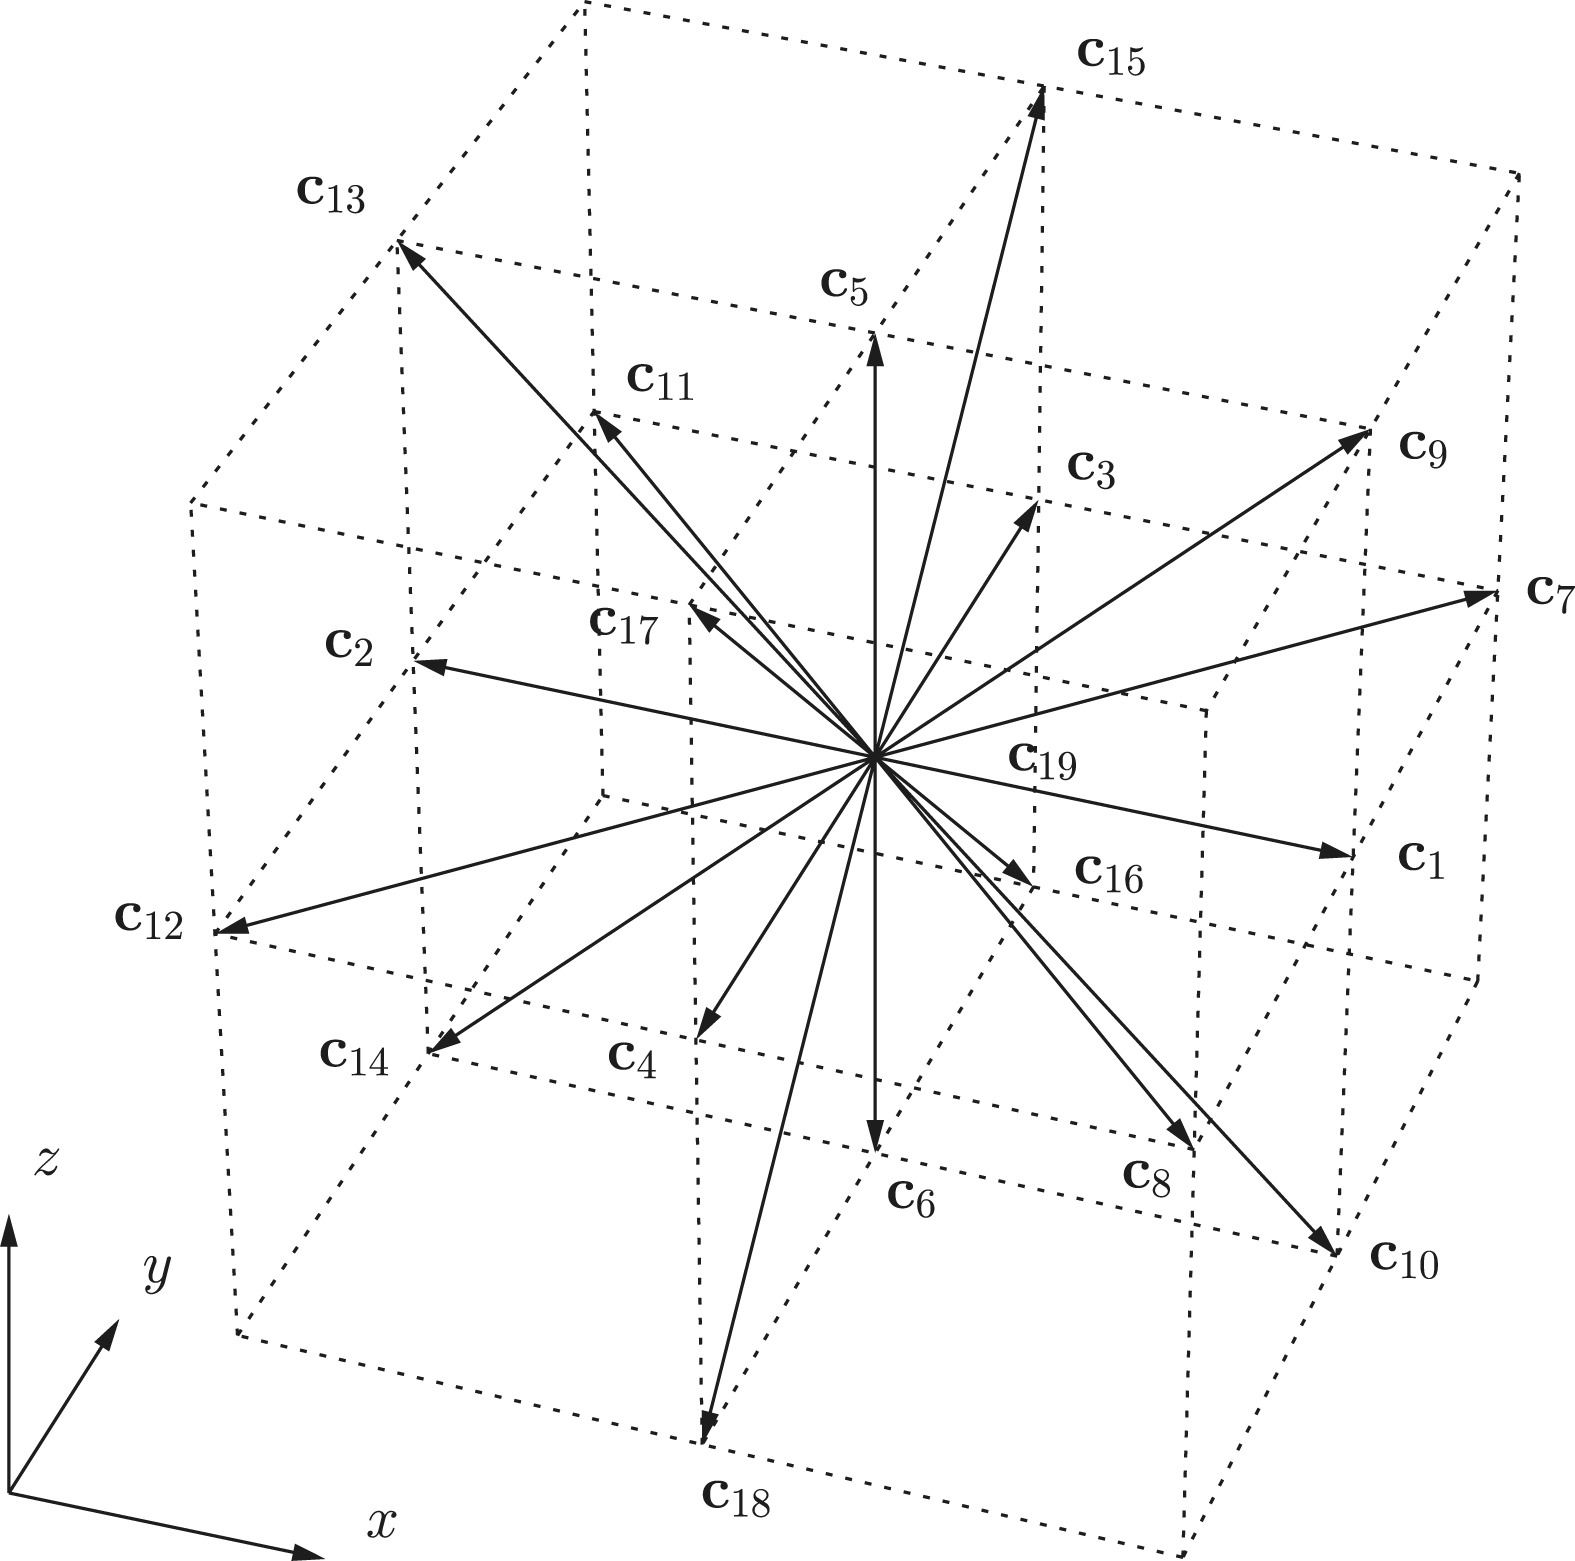
\includegraphics[scale = 0.7]{figures/methods/d3q19_lattice.jpg}
    \caption{D3Q19 lattice demonstrating the rest, nearest and next nearest direction that correspond to the 19 
    directions $(i)$ of the lattice with lattice velocity $c_{i}$. \cite{schmieschek_lb3d_2017} Reproduced from 
    Schmieschek et al. under the Creative Commons license.}
    \label{fig:d3q19_lattice}
\end{figure}

$\rho$ and $\textbf{u}$ in Equation \ref{eq:LBM_Feq} are defined as the macroscopic parameters for density and velocity 
and can be calculated from the mass distribution using $\rho = \sum f_i$ and $\rho \mathbf{u} = \sum f_i \mathbf{c}_i$ 
respectively. Using the Chapman-Enskog expansion, the Navier-Stokes equation at the incompressible limit at low mach
numbers can be recovered. \cite{qian_lattice_1992, he_lattice_1997} The regime accessible through this method is suitable 
for simulations in this work as the $ 1 \leq Re \leq 100 $ and the mach number, $Ma < 0.01$, fulfilling the stability 
criterion and usage requirements for the presented hydrodynamic model.

\section{Non-ideal mixing}
\label{section:lbm_non_ideal_mixing}

The SC model mimics Cahn-Hilliard type behaviour through a force applied from the other fluid species $k'$ in adjacent 
cells $\mathbf{x'}$ on fluid species $k$ at point $\mathbf{x}$. \cite{shan_lattice_1993, shan_simulation_1994, 
shan_multicomponent_1995, he_discrete_1998, jansen_bijels_2011, chin_lattice_2002} Both fluid species are defined
 by their own distribution equation defined in Equation \ref{eq:LBM_BGK} The strength of this force is controlled 
 through an interaction parameter, $g_{kk'}$ with no contribution from self interaction of the fluid as these are 
 set to zero. The SC force can then be written out in Equation \ref{eq:sc_model}.

\begin{equation}
% F_{k}^{SC}(\mathbf{x}, t) = -\Psi^{k}(\mathbf{x}, t)\sum_{k'}g_{cc'}\sum_{\mathbf{x'}}\Psi_{k'}(\mathbf{x'}, t)(\mathbf{x'} 
% - \mathbf{x})
\vec{F}_k(\vec{x}) \Delta t = - \sum_{k'} \sum_i \frac{w_i}{c_s^2} g_{kk'} \psi_k(\vec{x})\psi_{k'}(\vec{x}+\vec{c}_i) \vec{c}_i
\label{eq:sc_model}
\end{equation}

An effective mass of each fluid at node $\mathbf{x}$ is used in place of the actual density to scale it between zero 
and one and is defined as $\psi^{k}(\mathbf{x},t) = \rho_{0}\left[1 - \exp(-\frac{\rho^{k}(\mathbf{x}, t)}{\rho_{0}})\right]$. 
In this model, the SC force is incorporated into the macroscopic velocities that are then used to calculate the equilibrium
distribution $f_{i}^{k, eq}$ for fluid $k$, defined as,

\begin{equation}
\vec{u}_k^{\text{eq}} = \vec{u}' + \frac{\tau_k}{\rho_k} \vec{F}_k
\end{equation}

Where $\vec{u}'$ is defined as the common grid velocity and is calculated from $f_i^k$ below

\begin{equation}
    \sum_k \frac{\rho_k}{\tau_k} \vec{u}' = \sum_k \frac{1}{\tau_k}\sum_i f_i^k\vec{c}_i
\end{equation}

This recasting of the velocity ensures that in the absence of forces, the total momentum of the system is conserved. 

\section{Suspended particle dynamics}
\label{section:lbm_colloids}

Suspended particles will be coupled to the LB fluid based on the work conducted by Ladd. \cite{ladd_numerical_1994, 
aidun_direct_1998, ladd_lattice-boltzmann_2001} The particles follow Newtonian mechanics with the particle force and
rotational inertia defined using differential equations

\begin{equation}
    \begin{split}
    \vec{F_p} = m_p \frac{\vec{u}_p}{dt} , \\
    \vec{D_p} = \mathbf{J}_p \frac{\vec{\omega}_p}{dt} ,
    \label{eq:md}
    \end{split}
\end{equation}

$\mathbf{F_p}$ and $\mathbf{D_p}$ represent the force and torque acting on a particle with mass $m_p$ and moment of inertia 
$\mathbf{J}_p$. $\mathbf{u}_p$ and $\mathbf{\omega_{p}}$ are the linear and angular velocities of the particle. The equations of 
motion are evolved over time using a leapfrog integrator. \cite{jansen_bijels_2011}

The particles are discretized on the lattice according to the method laid out in Ladd and Aidun 
\cite{ladd_lattice-boltzmann_2001}. Nodes representing the particle are marked as solid nodes that replicate
a no-slip boundary condition through a moving bounce-back boundary. This is implemented into the distribution function
by reflecting the outgoing populations of $f_i^k$ to the opposite lattice velocity

\begin{equation}
    f^k_{i^\star}(\vec{x}, t+\Delta t) = f^{k,\star}_i(\vec{x}, t) - \frac{2w_i}{c_s^2} \rho \vec{u}_i \cdot \vec{c}_i ,
\end{equation}

This facilitates momentum exchange between particle and fluid which can be calculated analytically as 
\(\Delta\vec{p}^k_i \frac{\Delta t}{(\Delta x)^3} = 2 f^{k,\star}_i(\vec{x},t)\vec{c}_i - \frac{2w_i}{c_s^2}\rho(\vec{u}_i\cdot\vec{c}_i)\vec{c}_i\).
The sum of the momentum change across the surface of the particle is computed to obtain the force and torque on the particle,

\begin{equation}
    \begin{split}
    \vec{F}_p &= \sum_{k,i} \frac{\Delta \vec{p}^k_i}{\Delta t} , \\
    \vec{T}_p &= \sum_{k,i} \frac{\Delta\vec{p}^k_i}{\Delta t} \times \vec{r}_i .
    \end{split}
\end{equation}

As the particle moves, the nodes representing the particle are updated, with newly covered grid points marked as solid and 
uncovered nodes marked as fluid. When a grid point is covered, the momentum contained in that lattice point is added to the 
total force of the particle,

\begin{equation}
    \vec{F}_p = -\sum_{k,i} f_i^k(\vec{x},t)\vec{c}_i .
\end{equation}

Upon uncovering of a grid point, it is assigned a density value that represents the average of all adjacent fluid sites,

\begin{equation}
    \rho^k(\vec{x},t) = \frac{1}{N_{\text{f}}} \sum_{i_{\text{f}}} \rho^k(\vec{x}+\vec{c}_{i_{\text{f}}n}, t)
    \label{eq:fill_particles}
\end{equation}

\subsection{Anisotropic particles}
\label{section:lbm_colloids_ellipsoids}

For particles close to contact, meaning with inter-surface distances under 1 lattice unit the hydrodynamics are unresolved as the
distance is smaller than what the model can resolve. Lubrication forces are added to reduce the likelihood of particle overlap. For 
spherical particles, this is defined in Equation \eqref{eq:lubrication}

\begin{equation}
    \vec{F}_l = -6 \pi \eta \frac{R_1^2 R_2^2}{\left(R_1+R_2\right)^2}\left(\frac{1}{|\vec{r}_{ij}|-R_1-R_2}-\frac{1}{d_c}\right) \frac{\left(\vec{u}_{12}\cdot\vec{r}_{12}\right)\vec{r}_{12}}{|\vec{r}_{12}|^2} ,% \qquad d<d_c,
    \label{eq:lubrication}
\end{equation}

where $R_i$ and $R_j$ are the radii of each particle involved in the interaction, $\vec{r}_{ij}$ is the distance
vector between the particle centers, $\mathbf{u}_{ij}$ are the relative velocities of the particles and $\Delta_c$ 
is the cutoff distance when the lubrication force begins to act. If particles are able to overcome the lubrication forces, 
a hertzian contact force is also added to ensure that there is no particle overlap, defined in Equation \eqref{eq:hertz}

\begin{equation}
    \phi_{H} = K_{H}(R_i + R_j - |\mathbf{r}_{ij}|)^{5/2}, r < R_i + R_j
    \label{eq:hertz}
\end{equation}

$K_H$ is the force constant used to push particles apart. To correct for the anisotropic particles used in this work, 
the formulas presented in Eqs \ref{eq:lubrication} and \ref{eq:hertz} can be generalized using the route followed 
in Gunther et al. and Davies et al., inspired by Berne and Pechukas. \cite{gunther_timescales_2014, davies_interface_2014} 
They first begin by rewriting the lubrication and Hertzian contact forces as a function of the particle orientation and 
aspect ratio of the particles.

\begin{equation}
    \begin{split}
    \phi(\vec{r}_{ij}) &= {\epsilon} \tilde{\phi}\left(\frac{\vec{r}_{ij}}{{\sigma}}\right) , \\
    \vec{F}(\vec{r}_{ij}) &= {\epsilon} \tilde{\vec{F}}\left(\frac{\vec{r}_{ij}}{{\sigma}}\right) .
    \end{split}
\end{equation}

For the lubrication force \eqref{eq:lubrication}, we choose
${\sigma}=R_1+R_2$ and ${\epsilon}=\frac{6\pi\eta R_1^2 R_2^2}{{\sigma^3}}$, and for the
Hertz potential we chose ${\sigma}=R_1+R_2$ and ${\epsilon}=K_H\sigma^{5/2}$. For two identical, rotationally
symmetric ellipsoidal particles with orientations $\hat{\vec{o}}_i$ and $\hat{\vec{o}}_j$, we then replace $\epsilon$ and $\sigma$ by
the anisotropic functions

\begin{equation}
    \begin{split}
    \tilde\epsilon\left(\hat{\vec{o}}_i, \hat{\vec{o}}_j\right) &= \frac{{\epsilon}}{\sqrt{1-\chi^2}} , \\
    %\qquad \chi = \frac{\left(\alpha^2-1\right)R_\parallel^2}{\left(\alpha^2+1\right)R_\parallel^2}\left(\hat{\vec{o}}_i\hat{\vec{o}}_j\right) , \\
    \tilde\sigma\left(\vec{r}_{ij}, \hat{\vec{o}}_i, \hat{\vec{o}}_j\right) &= \frac{{\sigma}}{\sqrt{1-\frac{\chi}{2}\left[ \frac{\left(\hat{\vec{r}}_{ij}\cdot\hat{\vec{o}}_i+\hat{\vec{r}}_{ij}\cdot\hat{\vec{o}}_j\right)^2}{1+\chi\left(\hat{\vec{o}}_i\hat{\vec{o}}_j\right)} + \frac{\left(\hat{\vec{r}}_{ij}\cdot\hat{\vec{o}}_i-\hat{\vec{r}}_{ij}\cdot\hat{\vec{o}}_j\right)^2}{1-\chi\left(\hat{\vec{o}}_i\hat{\vec{o}}_j\right)} \right] }} , \\
    \chi &= \frac{\alpha^2-1}{\alpha^2+1} , \\
    \end{split}
\end{equation}

where $R_{\parallel}$ is the particle radius along the
symmetry axis $\hat{o}$ and $\alpha=\frac{R_{\parallel}}{R_{\perp}}$ the aspect
ratio of the particle. The anisotropic Hertz potential and lubrication
force are then defined as
%
\begin{equation}
    \begin{split}
    \phi\left(\vec{r}_{ij}, \hat{\vec{o}}_i, \hat{\vec{o}}_j\right) &= \epsilon\left(\hat{\vec{o}}_i, \hat{\vec{o}}_j\right) \tilde{\phi}\left(\frac{\vec{r}_{ij}}{\sigma\left(\vec{r}_{ij}, \hat{\vec{o}}_i, \hat{\vec{o}}_j\right)} \right) , \\
    \vec{F}\left(\vec{r}_{ij}, \hat{\vec{o}}_i, \hat{\vec{o}}_j\right) &= \epsilon\left(\hat{\vec{o}}_i, \hat{\vec{o}}_j\right) \tilde{\vec{F}}\left(\frac{\vec{r}_{ij}}{\sigma\left(\vec{r}_{ij}, \hat{\vec{o}}_i, \hat{\vec{o}}_j\right)} \right) .
    \end{split}
\end{equation}

\subsection{Magnetic field and particle coupling}
\label{section:lbm_colloids_magnetics}

The magnetic dipole potential is defined as

\begin{equation}
    \mathbf{U_{ij}} = \frac{\mu_0 m_i m_j}{4\pi r_{ij}^{3}} \left[ \Hat{\mathbf{o_i}} \cdot \Hat{\mathbf{o_j}} - 
    3(\Hat{\mathbf{o_i}} \cdot \Hat{\mathbf{r_{ij}}})(\Hat{\mathbf{o_j}} \cdot \Hat{\mathbf{r_{ij}}}) \right]
    \label{eq:magnet_potential}
\end{equation}

Where $\mu_0 = 4\pi \cdot 10^{-7} \frac{H}{m}$,  $\Hat{\mathbf{o_i}}$ is the orientation unit vector of particle 
$i$, $\Hat{\mathbf{r_{ij}}}$ is the distance vector between particles $i$ and $j$ and $m_i$ is the magnitude the 
magnetic dipole of particle $i$. From the potential, the force and torque of the dipole force between particles 
can be found. These expressions are shown in equations \ref{eq:dipole_magnetic_force} and \ref{eq:dipole_magnetic_torque} 
for the force and torque respectively.

\begin{equation}
    \mathbf{F}_{ij} = \frac{3 \mu_0}{4 \pi} [\frac{5(m_i \cdot \mathbf{r}_{ij})(m_j 
    \cdot \mathbf{r}_{ij})}{|\mathbf{r}_{ij}|^7}\mathbf{r}_{ij} - \frac{(m_i \cdot m_{j})\mathbf{r}_{ij} + 
    (m_i \cdot \mathbf{r}_{ij})m_i + (m_j \cdot \mathbf{r}_{ij})m_j }{|\mathbf{r}_{ij}|^5}]
\label{eq:dipole_magnetic_force}
\end{equation}

\begin{equation}
    \mathbf{T}_{ij} = \frac{\mu_0}{4 \pi}[ \frac{3(m_j \cdot \mathbf{r}_{ij})m_i \times \mathbf{r}_{ij} }
    {|\mathbf{r}_{ij}|^5} - \frac{m_i \cdot m_j }{|\mathbf{r}_{ij}|^3} ]
    \label{eq:dipole_magnetic_torque}
\end{equation}

Equations \ref{eq:magnet_force} and \ref{eq:magnet_torque} are used to calculate the force and torque that the 
field exerts on each particle.

\begin{equation}
    \mathbf{F_{j}} = (m_j \Hat{\mathbf{o_j}} \cdot \nabla B_i)
    \label{eq:magnet_force}
\end{equation}

\begin{equation}
    \mathbf{\tau_j} = (m_j \Hat{\mathbf{o_j}} \times B_i)
    \label{eq:magnet_torque}
\end{equation}

The total force and torque exerted on each particle is the sum of the particle dipole interaction and the field 
dependent contribution. 